\documentclass{beamer}
\usetheme{Warsaw}
\useinnertheme{circles}
\useoutertheme[subsection=false]{smoothbars}
\usepackage[utf8x]{inputenc}
\usepackage[czech]{babel}
\usepackage[T1]{fontenc}
\usepackage{listings}
\usepackage{tikz}
\lstset{basicstyle=\tiny\ttfamily}
\logo{
\includegraphics[height=0.5cm]{brmlab.pdf}}

\begin{document}

\AtBeginSection[]
{
  \begin{frame}
    \frametitle{Outline}
    \tableofcontents[currentsection]
  \end{frame}
}

\title{brmiversity: Umělá inteligence \\ a teoretická informatika}
\subtitle{Přednáška č. 11}
\author{Petr Baudiš $\langle${\tt pasky@ucw.cz}$\rangle$}
\institute{
	brmlab 2011\\
	\vskip 1ex
	\pgfdeclareimage[height=4ex]{ccbysa}{by-sa.pdf}
	\pgfuseimage{ccbysa}
}
\date{}
\frame{\titlepage}

\section{Neuronové sítě}

\subsection{}
\begin{frame}{Samoorganizace pomocí ANN}
\begin{itemize}
\item Umělé neurony (``výpočetní krabičky'') \\ dostávají vstupy (čísla) a na jejich \\ základě generují výstup (číslo)
\item Dnes: ``Jedna'' vrstva, chceme asociovat \\ různé vstupy s různými neurony
\item Učení bez učitele --- redukci (s určitými parametry) najdi sám
\item Učení s učitelem --- redukuj podle předložených tříd
\end{itemize}
\begin{tikzpicture}[remember picture,overlay]
  \node [xshift=-4.5cm,yshift=-5cm,above right] at (current page.north east)
    {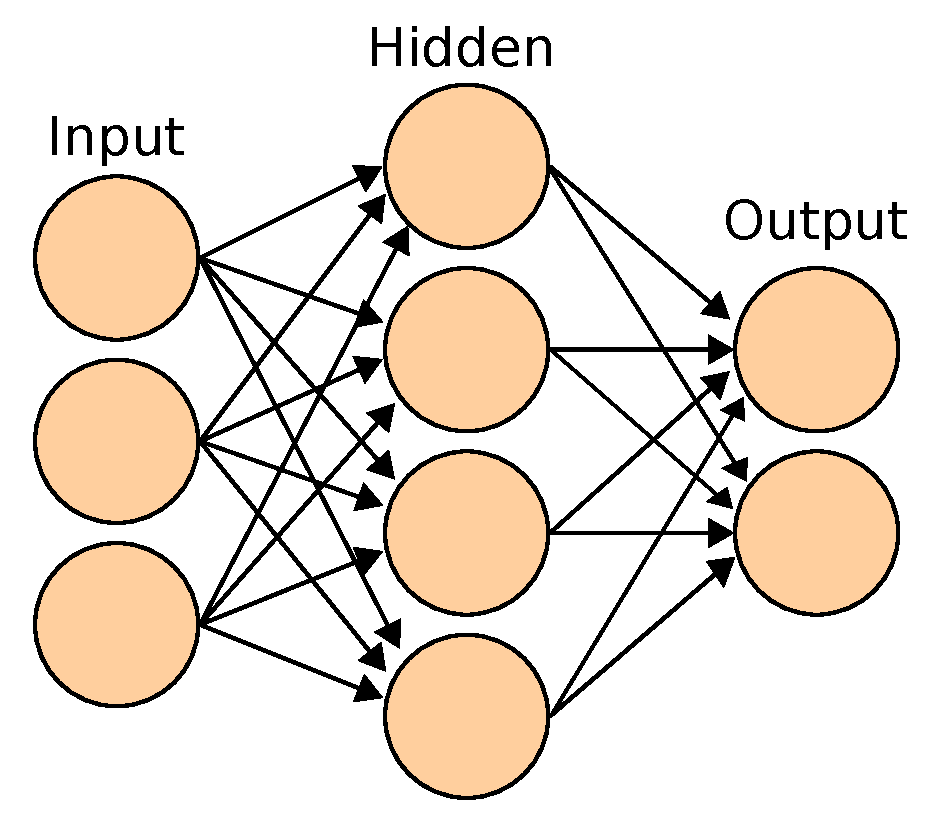
\includegraphics[width=4cm]{ANN.pdf}};
\end{tikzpicture}
\end{frame}

\subsection{}
\begin{frame}{Kompetiční učení}
\begin{itemize}
\item Neurony soutěží o vzory; váhový vektor $\vec w$ odpovídá pozici v~prostoru vzorů
\item {\bf Vítěz bere vše:} Vítěz je právě jeden nejbližší neuron
\item {\bf Adaptace:} Vítězný neuron posuneme směrem k vzoru $$\vec w' = \vec w + \alpha \cdot (\vec x - \vec w)$$
\item ({\bf Laterální inhibice:} Okolní neurony odsuneme \\ směrem {\em od} vzoru)
\vskip 3ex
\item Připomíná vám to něco? \pause $k$-means shlukování!
\item Lze dokázat, že konverguje ke $k$-means a při dobře ohraničených shlucích je stabilní
\item Tvar shluku je omezen lineárním klasifikátorem
\item Lepší stabilita: dávková aktualizace
\end{itemize}
\end{frame}

\subsection{}
\begin{frame}{Kohonenova mapa}
\begin{itemize}
\item Uspořádání výstupních neuronů je důležité (třeba 2D mřížka)
\item Tedy: $n$-rozměrný vstupní prostor (kombinace $n$ vstupních neuronů) redukujeme do $k$-rozměrného výstupního prostoru
\item Spatiální koherence: Vzory blízko ve vstupním prostoru by měly zůstat blízko ve výstupním (a naopak?)
\vskip 3ex
\item Fonetický ``psací stroj'', ekonomická data, politická data
\end{itemize}
\end{frame}

\subsection{}
\begin{frame}{Kohonenova mapa}
\begin{center}
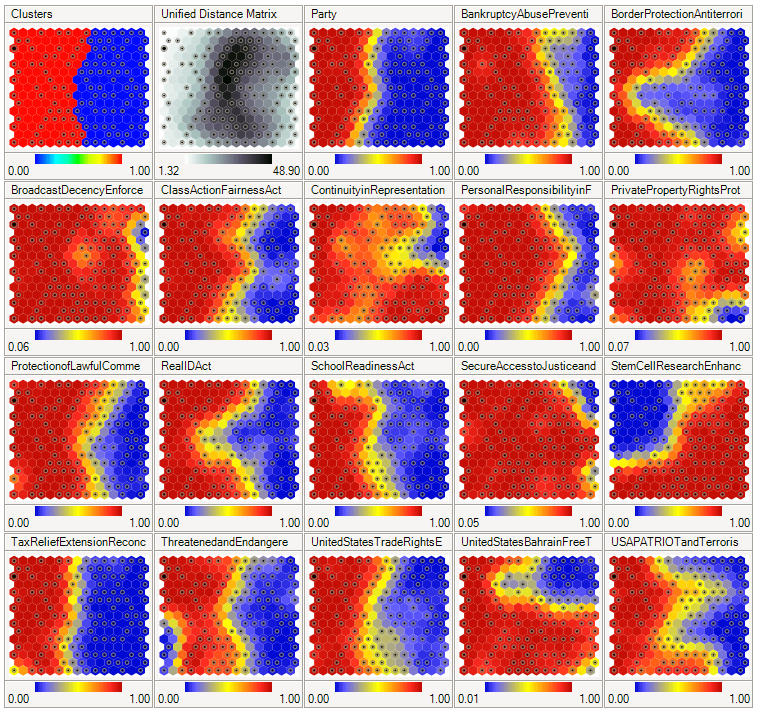
\includegraphics[width=8cm]{Synapse_Self-Organizing_Map.png}
\end{center}
\end{frame}

\subsection{}
\begin{frame}{Kohonenova mapa}
\begin{itemize}
\item Váhový vektor $\vec w$ neuronu odpovídá jeho \\ pozici ve vstupním prostoru
\item Vzdálenost vstupu k neuronu $j$: $d_j = \sum_{i=1}^k (x_i - w_{ij})^2$
\item Vybavení: Vyber nejbližší neuron ($\mathrm{argmin}_j \,  d_j$)
\pause
\vskip 3ex
\item Neurony jsou rozmístěny v euklidovském prostoru, \\ každý neuron má okolí dané poloměrem $r$
\item Funkce laterální interakce $\Phi(a,b)$ --- síla propojenosti \\ neuronů $a$ a $b$, obvykle klesá se vzdáleností
\item Učení: Vyber nejbližší neuron $c$, neurony v okolí $r$ posuň
	$$ w_{ij}' = w_{ij} + \alpha(t) \cdot \Phi(c, j) \cdot (x_i - w_{ij}) $$
	$\alpha(t)$ klesá s časem
\item Lze dokázat konvergenci
\end{itemize}
\end{frame}

\subsection{}
\begin{frame}{Lateral Vector Quantization}
Učení s učitelem --- máme definované {\em třídy} $c(\vec x)$

$\vec x$ by měl patřit ke stejné třídě jako nejbližší $\vec w$

\begin{block}{Adaptační pravidlo LVQ1}
\begin{itemize}
\item Adaptujeme pouze vítězný (nejbližší) neuron:
\item $c(\vec x) = c(\vec w_j)\colon w_{ij}' = w_{ij} + \alpha(t) \cdot (x_i - w_{ij})$
\item $c(\vec x) \ne c(\vec w_j)\colon w_{ij}' = w_{ij} - \alpha(t) \cdot (x_i - w_{ij})$
\end{itemize}
\end{block}
\end{frame}

\subsection{}
\begin{frame}{Adaptační pravidlo LVQ2.1}
\begin{itemize}
\item Adaptujeme dva nejbližší neurony; soustředíme se na {\em posouvání hranic oblastí}
\item Buď $j,k$ nejbližší neurony; učíme se pouze pokud \\ $j$ má správnou třídu, $k$ špatnou třídu
\item Zároveň $x$ je z ``okénka'', na rozhraní $i$ a $j$ ve vstupním prostoru (okolí dělící nadroviny $\vec w_i$ a $\vec w_j$)
\vskip 3ex
\item $w_{ij}' = w_{ij} + \alpha(t) \cdot (x_i - w_{ij})$
\item $w_{ik}' = w_{ik} - \alpha(t) \cdot (x_i - w_{ik})$
\item LVQ3: $w_{ik}' = w_{ik} + \varepsilon \cdot \alpha(t) \cdot (x_i - w_{ik})$, \\ je-li $k$ také správná třída (stabilizace řešení)
\end{itemize}
\end{frame}

\subsection{}
\begin{frame}{Další metody samoorganizace}
\begin{itemize}
\item Sítě se vstřícným šířením (TODO: Grossbergovská vrstva?)
\item Adaptive Resonance Theory (ART): Laterální inhibice, TODO
\item PCA pomocí posilovaného učení lineárního klasifikátoru (neuronu) --- Ojův algoritmus
\end{itemize}
\end{frame}

\subsection{}
\begin{frame}{Otázky?}
\begin{center}
Příště: Modulární, hierarchické a hybridní modely.
\end{center}
\end{frame}

\section{Adaptivní agenti}

\subsection{}
\begin{frame}{Etologické modely}
\begin{columns}
\begin{column}{6cm}
\begin{itemize}
\item Analytické vs. simulační modely
\item Emergentní chování
\item Akční patterny; apetitivní chování; konzumační chování
\item Lorenzův psychohydraulický model
\item V umělých bytostech Tyrrellova free-flow hierarchie (už bylo)
\end{itemize}
\end{column}
\begin{column}{5cm}
Non-free artwork omitted. See
\url{http://terpconnect.umd.edu/~wrstrick/secu/ansc455/model.gif}
%\includegraphics[width=5cm]{model.png}
\end{column}
\end{columns}
\end{frame}

\subsection{}
\begin{frame}{Populační dynamika}

\begin{block}{Rozmnožování}
\begin{itemize}
\item Fibonacciho posloupnost $F_{i+2} = F_{i+1} + F_i$ (množení králíků)
\item Logistická funkce: $dN/dt = rN(1-N/K)$
\item $r$ je rychlost množení, $K$ je kapacita prostředí; \\ $r$-stratég vs. $K$-stratég
\item Řešení $1 \over 1 + e^{-t}$ resp. $KP_0e^{rt} \over K+P_0(e^rt-1)$
\end{itemize}
\end{block}

\begin{block}{Model predátor-kořist}
\begin{itemize}
\item Dynamický systém Lotka-Volterra
\item $dx/dt = x(\alpha - \beta y) \qquad dy/dt = -y(\gamma - \delta x)$
\item $y$ jsou predátoři, $x$ je kořist
\item Rovnovážné stavy nebo cykly, např. $\{y=\alpha/\beta, x = \gamma/\delta\}$
\item Obecněji Kolmogorovské modely
\end{itemize}
\end{block}
\end{frame}

\subsection{}
\begin{frame}{Otázky?}
\begin{center}
Příště: Reprezentace znalostí.
\end{center}
\end{frame}

\section{Evoluční algoritmy}

\subsection{}
\begin{frame}{Koevoluce}
\begin{itemize}
\item Populace problémů a populace řešítek
\item Paralelní vývoj problémů i řešení
\item Fitness řešítka: Procento vyřešených problémů
\item Fitness problému: Procento selhávajících řešítek
\vskip 3ex
\item Analogie s parazity (červená královna)
\item Třídící sítě
\item Knihovna zahájení v Go
\item Evoluční teorie her
\item Umělý život
\end{itemize}
\end{frame}

\subsection{}
\begin{frame}{Otevřená evoluce}
\begin{itemize}
\item Strop fitness je (skoro?) nekonečno!
\item Typicky umělý život (fact-free science)
\item Fitness je endogenní --- obvykle přežití (rozmnožení) nebo smrt
\vskip 3ex
\item Core Wars (evoluce v principu neprobíhá)
\item Tierra, Avida (soutěž i o zdroje jako CPU, samozměny)
\item Evolve (celulární automat)
\item DigiHive (částice, konzistentní fyzikální model)
\item Framsticks, breve (3D model světa)
\item Brmlife
\vskip 3ex
\item Skutečně otevřená evoluce --- otevřený problém
\end{itemize}
\end{frame}

\subsection{}
\begin{frame}{Pravděpodobnostní model GA}
\begin{itemize}
\item Opět trocha suché teorie, jak GA funguje
\item Vzorečky: Pravděpodobnost vzniku schématu,
	sledujeme vývoj fitness jako dynamický systém
\item Jak GA funguje? Stejně nevíme!
\end{itemize}
\end{frame}

\subsection{}
\begin{frame}{Otázky?}
\begin{center}
Příště: Hrst aplikací.
\end{center}
\end{frame}

\section{Složitost}

\subsection{}
\begin{frame}{Třídy složitosti}
\begin{itemize}
\item Rekapitulace --- P, NP, PSPACE, EXPTIME
\end{itemize}
\end{frame}

\subsection{}
\begin{frame}{Míry složitosti}
\begin{itemize}
\item Polynomiální hierarchie
\end{itemize}
\end{frame}

\subsection{}
\begin{frame}{Savičova věta}
\begin{itemize}
\item TODO
\end{itemize}
\end{frame}

\subsection{}
\begin{frame}{Konstruovatelné funkce}
\begin{itemize}
\item TODO
\end{itemize}
\end{frame}

\subsection{}
\begin{frame}{Věty o zrychlení a mezerách}
\begin{itemize}
\item TODO
\end{itemize}
\end{frame}

\subsection{}
\begin{frame}{Hierarchie tříd složitosti}
\begin{itemize}
\item TODO
\end{itemize}
\end{frame}

\subsection{}
\begin{frame}{Otázky?}
\begin{center}
Příště: Pseudopolynomiální a aproximační algoritmy.
\end{center}
\end{frame}

\subsection{}
\begin{frame}{Děkuji vám}
\begin{center}
{\bf pasky@ucw.cz}

\vskip 6ex

Příště: Umělá inteligence a adaptivní agenti (reprezentace znalostí). \\
	Neuronové sítě.
	Evoluční algoritmy. \\
	Vyčíslitelnost (algoritmicky nerozhodnutelné problémy).
\end{center}
\end{frame}

\end{document}
